\documentclass{article}
\usepackage[utf8]{inputenc}
\usepackage{natbib}
\usepackage{hyperref}
\usepackage{listings}
\usepackage{graphicx}

\begin{document}

\title{INFO2222 Assignment 1}
\author{Mingyuan Ba}
\date{\today}
\maketitle

%======================================================================

\section{Part1}
\subsection{Q1}
\begin{enumerate}
    \item Web server handling online sales for the computer hardware parts.
        \begin{itemize}
            \item \textbf{Confidentiality}: In this scenario,this principle need to ensures that sensitive data is accessible only to those authorized users\cite{Lecture1}. A possible solution to this is encrypting data transmission using protocols like SSL, which helps in securing user data.
            \item \textbf{Integrity}: This principle ensures that information keeps accurate during transmission\cite{Lecture1}. It can be implemented by using hash function\cite{2-1-1.Hash(1)} and digital signature to validate the integrity of the data transmitted.
            \item \textbf{Availability}: This principle ensures that users have reliable access to the website and do operations when needed\cite{Lecture1}. Techniques to achieve availability include setting up load balancer\cite{AlibabaCloud2019HighAvailability}, and utilizing robust hardware resources, ensuring that users can do operations when needed.
        \end{itemize}
        
    \item ATM machines
        \begin{itemize}
            \item \textbf{Confidentiality}: This principle ensures that only authorized users and systems can access transaction details and user data\cite{Lecture1}. It can be implemented by encrypting data transmission to secure customer PINs and transaction data from unauthorized access.
            \item \textbf{Integrity}: This principle ensures that transaction information remains accurate during its transmission and processing\cite{Lecture1}. In this scenario,Secure Socket Layer (SSL) and Transport Layer Security (TLS) \cite{TritonSSLProject}protocols not only provide an encrypted connection from the ATM to the host, protecting the data from leaks, but also ensure the integrity of the data during transmission.
            \item \textbf{Availability}: This principle guarantees that customers can access services like withdrawals anytime they need\cite{Lecture1}. To ensure continuous operation, ATMs can be equipped with backup power supplies and multiple network connections to handle hardware failures or network issues efficiently.
        \end{itemize}
\end{enumerate}

\subsection{Q2}
	Reasons:
	\begin{enumerate}
		\item To use one-time pad, both the sender and receiver need to have the same key.But the issue is that if the key is compromised during transmission, the security of the encryption can not be promised.\\\\
		\textit{Example}:\\
		Suppose that James and Alex are in Sydney and Melbourne separately.If they send key via internet or e-mail,the key could be intercepted by a third party during transit.Once the key is compromised, the security of the communication can no longer be guaranteed.

		\item Since the key used in a one-time pad must have the same length of the message, managing and storing such long keys becomes hard.
		\textit{Example}:\\
		If Rubin needs to send many large files to James, ensuring the keys are sent and managed correctly and securely would be a significant challenge for both parties.

		\item The encryption and decryption process in a one-time pad is bit-by-bit, which can be computationally expensive and slow for large amounts of data.

		\textit{Example}:\\
		Suppose that Alex wants to send a large 5GB file to Rubin using a one-time pad.This means for a 5GB file, they would need a key that is also 5GB in size, which equates to 40 billion bits. This process involves operating on every single bit of the file, resulting in an encrypted file of the same size.

	\end{enumerate}
	Therefore, while the one-time pad provides perfect secrecy, it is not practical for most scenarios.\\

\newpage
	\textbf{\textit{Stream ciphers}} are encryption algorithms that encrypt and decrypt messages by applying a cryptographic key and algorithm to each binary digit in a data stream, one bit at a time\cite{OktaStreamCipher}.

    \begin{figure}[htbp]
        \centering % 图片居中
        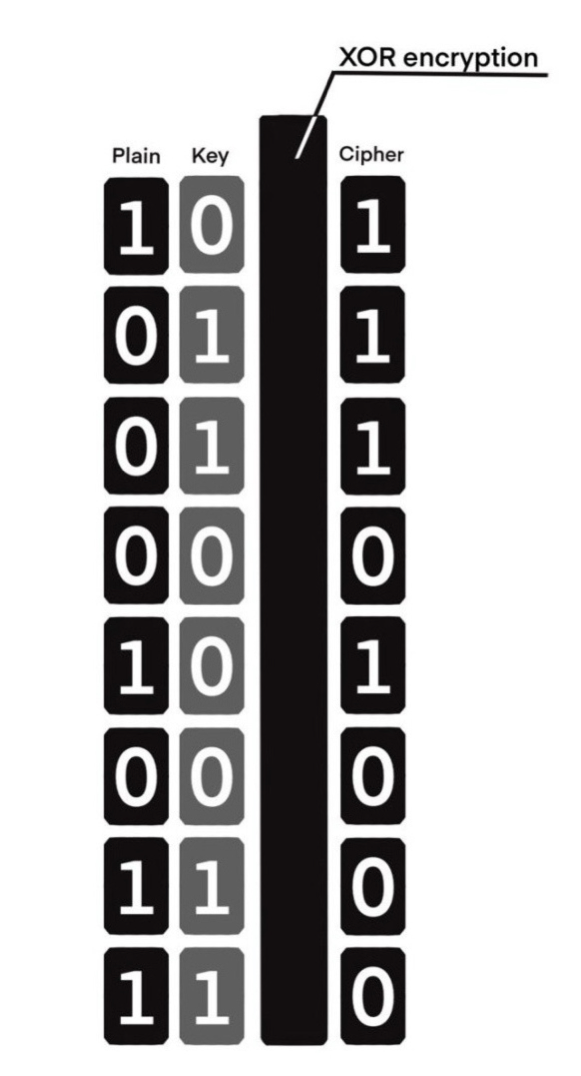
\includegraphics[width=0.3\textwidth]{graphs/Stream_cipher.jpg} 
    \end{figure}

	\textbf{\textit{Pseudorandom generators}} are needed with stream ciphers to stretch a short key and generate a longer sequence of pseudorandom bits\cite{3-1.Symmetric-Crypto}. 


\subsection{Q3}
	The main difference between hash functions and MACs is that hash functions don't require a key for their operation. Hash functions produce a hash value for any input without a key. On the other hand, MACs use a secret key alongside data to produce a tag.It ensures the authenticity and integrity of the message for sender\cite{3-1.Symmetric-Crypto}.

	\begin{lstlisting}[language=Python]
	# By Hash
	digest = Hash(M)

	# By MACS
	digest = MACS(M,key)
	\end{lstlisting}

	HMAC combines the properties of hash functions and MACS. HMAC uses a cryptographic hash function along with a secret key to generate a tag. This tag can be verified by the recipient using the same secret key and hash function. The use of a secret key makes HMAC more secure as it adds an additional protection against .

	\begin{lstlisting}[language=Python]
	# By HMAC 
	K1 = preprocess_key(key)
	K2 = preprocess_key(key)
	inner_digest = Hash(K1 | M)
	digest = Hash(K2 | inner_digest)
	\end{lstlisting}

	Using 2 keys in HMACS for internal and external hash isolates these processes.Even though the inner hash were compromised by third parties,they can not produce a digest to deceive the receiver without external key.

	Compared to MACs, using HMAC for secure communication is like sending a locked box to someone, but with two keys. First, you use a secret code (K1) to lock the box inside another box. Then, you use a different secret code (K2) to lock the outer box. Even if someone figures out the first code (K1), they can't open the outer box without the second code (K2).

	Besides,these two hash operations secure HMAC against a length extension where atttacker can add additional data to a message and generate a valid new hash value without knowing the original message content, only its hash\cite{Length_extension_attack}.

	The shortcomings of hash are the collision resistance and pre-image attacks\cite{2-1-1.Hash(1)}.It is possible for two different messages to produce the same hash output, although the probability is extremely low.Pre-image attack involves attempting to reverse the hash function to determine the original input that generated a particular hash.

	In HMAC or MAC, both the sender and the receiver have to know the key .This means that when sharing the key over the internet, it could be stolen by a third party.


\subsection{Q4}

In SHA-256, the number "256" refers to the bitsize of the output\cite{SSLDragonSHA256}.

SHA-1 is considered "broken" for collision resistance \cite{2-1-1.Hash(1)}, meaning that it is possible to find two different inputs that produce the same hash value. This property makes SHA-1 unsuitable for secure applications. In contrast, SHA-256 provides higher performance in collision resistance.\\\\


\textbf{\textit{Differences}} between SHA-256 and MD5
\begin{itemize}
	\item MD5 produces output faster than SHA256. SHA256 is slower than MD5 because of its complex algorithm and larger output size\cite{9573660}.

	\item MD5 is broken and insecure for cryptographic use because collision attacks can efficiently produce the same hash for different inputs\cite{2-1-1.Hash(1)}. On the contrary, SHA256 is more secure against such attacks.
\end{itemize}

\textbf{\textit{Example}}

	\begin{lstlisting}[language=Python]
	# Suppose s is a string with 1000000 characters

	# Hash by MD5
	md5_hash = hashlib.md5(s.encode()).hexdigest()

	# Hash value: 174ac9a4f023a557a68ab0417355970e

	# Hash by sha-256
	sha256_hash = hashlib.sha256(s.encode()).hexdigest()

	# Hash value: ec21d64624228af3ecd4bdaa8239e32ed943b01e26934cd5610fddb361426dc6
	\end{lstlisting}

	As the example shown above demonstrates, SHA-256 produces a longer hash output and is more secure against collision attacks.

\subsection{Q5}

	To achieve this, USYD can utilize a Key Derivation Function (KDF) to generate unique keys for students from the master key without the need to store each one. The KDF combines the master key and the SID to generate a unique key\cite{adams2004security}, which each student can use to access Canvas. This method ensures that even if a student's key is compromised, both the master key and the keys of other students remain secure.


\section{Part2}

\subsection{Q1}

	\begin{enumerate}
		\item Due to the independence of each attempt, the probability can be calculated by summing the probabilities of each time:
		\begin{center}
			$6 \cdot \frac{1}{10000} = \frac{6}{10000}$
		\end{center}

		\item 
		\begin{enumerate}
	    \item \textbf{Identify Alice's Entry}: A locates the database entry corresponding to Alice, identified by her name and the hash of her password (name; H(pwd)).
	    \item \textbf{Understand the Hash Function}: A needs to figure out which hash function are used by the email server(e.g. sha-256).
	    \item \textbf{Use a Rainbow Table or Dictionary Attack}: Since hash functions are irreversible, A can use pre-computed tables, known as rainbow tables, which contain a large number of plaintext passwords and their corresponding hash values, to find a match for the hash value (name; H(pwd)) associated with Alice's password\cite{4_Identification}. If the hash function used includes salt (a random value added to the password before hashing), this approach becomes much more challenging. A dictionary attack involves trying many passwords to see if they match.
	    \item \textbf{Reconstruct the Password}: Once A finds a match for the hash value using one of the methods above, they can reconstruct Alice's password with 100\% confidence.
	\end{enumerate}
\end{enumerate}

\subsection{Q2}

	\begin{itemize}
		\item \textbf{Advantages}
		\begin{enumerate}
			\item \textit{Convenience}: Biometrics such as fingerprints and facial recognition allow for quick identity verification through simple body movement,which typically completed in just a few second,while password verification usually takes longer time.Besides,users don't need to remember passwords or change them regularly to ensure security.

			\item \textit{Security}:Compared with password verification, it is nearly impossible to replicate due to its uniqueness, unlike passwords which can be replicated.
		\end{enumerate}

		\item \textbf{Disadvantages}
		\begin{enumerate}
			\item \textit{Irreversibility}: Once a biometric attribute (e.g., fingerprint, iris pattern) is compromised, it cannot be easily changed or reset like a password.
			\item \textit{Error Rates}: Biometric systems can mistakenly accept the wrong person or reject the right person. This mistake rate can change due to the technology, surroundings, or changes in a person's biometric features over time, leading to security risks or trouble accessing the system\cite{o2003comparing}.
		\end{enumerate}


	\end{itemize}


\subsection{Q3}

	\begin{itemize}
		\item \textbf{something you have}: 
		The advantage is its physical security. Even if someone knows your password or personal details, they still can't access your account without the physical item. This method adds an additional layer of security, decreasing the risk of unauthorized access.

		\item \textbf{someone you know}:
		The benefit lies in convenience and not needing to remember passwords or carry physical items. It uses social networks for authorization, offering an easy way to regain access through known contacts.s.

	\end{itemize}

\subsection{Q4}

	\begin{enumerate}
		\item \textbf{Q1}: 

		During the TLS handshake phase, digital certificates and server authentication are used to prevent impersonation. In this process, the server presents its digital certificate, which is issued by a Certificate Authority (CA) and includes the server's public key. The client verifies the authenticity of the certificate by checking the digital signature against the CA's public key.

		If the certificate is deemed valid and trustworthy, the client can be assured that it is communicating with the actual server. This procedure relies on the fact that attackers cannot forge a valid certificate signed by a trusted CA, nor can they obtain the private key. Thus, without using a pre-master secret, the core of the entire process lies in the role of the CA and the verification of digital certificates

		\item \textbf{Q2}:
		In TLS, each session generates a new random nonce as a nonce and uses it together with the key\cite{5-2.security-protocol}. This means that even if an attacker replays a previously eavesdropped session, the message will be encrypted into a different ciphertext due to the use of a new random nonce and key, making it impossible to decrypt into the original message. 

		\item \textbf{Q3}:
			\begin{itemize}
				\item \textit{SQL injections}: TLS/SSL does not protect against SQL injections, which are a type of attack where an attacker inserts malicious SQL code into a query, allowing them to manipulate or retrieve sensitive data from a database\cite{5-2.security-protocol}.

				\item \textit{Client/Server side vulnerabilities}: TLS/SSL cannot protect against vulnerabilities in the client or server applications themselves\cite{5-2.security-protocol}. If either the client or server has a vulnerability, an attacker can exploit it to gain unauthorized access or manipulate data, regardless of the TLS/SSL encryption in place.
			\end{itemize}

	\end{enumerate}

\section{Q3}

\subsection{Q1}
	\begin{enumerate}
		\item \textbf{Q1}:
		Virus signatures help detect and identify malware like viruses\cite{Lenovo2023VirusSignature}. Each virus has unique code features, and these signatures mark those features. By comparing these signatures with file codes, antivirus software can spot and block these threats, quickly protecting against known dangers.

		\item \textbf{Q2}:
		\textbf{Key methods:}
			\begin{itemize}
				\item \textbf{Polymorphism}: This technique involves the virus changing its code or payload with each infection, making it difficult for antivirus software to recognize the virus based on signatures or predefined patterns. Since most antivirus solutions rely on databases of known virus signatures to detect threats, a polymorphic virus can bypass detection by presenting a new signature each time it infects a new system.

				\item \textbf{Obfuscation and Encryption}: Some viruses are designed to encrypt or obfuscate their code in such a way that makes it hard for antivirus programs to analyze and identify the malicious code. This can involve the use of complex encryption algorithms or the insertion of irrelevant code (known as "dead code") to confuse the antivirus software's scanning and heuristic analysis techniques.
			\end{itemize}

		\textbf{What should we do being an antivirus organization}
			\begin{itemize}
				\item \textbf{Regularly Update Virus Definitions}: Ensure that the virus signature database is updated frequently with information about the latest threats. This requires a dedicated research team that constantly monitors new threats and develops signatures for them.

				\item \textbf{Encourage Community Reporting}: Create a platform for users and security researchers to report new threats and share information about potential vulnerabilities. This community-driven approach can help in quickly identifying and responding to new virus outbreaks.
			\end{itemize}
	\end{enumerate}

\subsection{Q2}
	\begin{enumerate}
		\item \textbf{Security Vulnerabilities:} Granting permissions like "Send SMS messages" and "Access your address-book" can expose your smartphone to security vulnerabilities. Malicious apps could exploit these permissions to conduct scam operations, send malware-infected links via SMS, or even use your device as part of a botnet without your knowledge.

		\item \textbf{Personal Data Exploitation:} These permissions can lead to the exploitation of personal data. For instance, access to your address book can enable an app to collect sensitive information about you and your contacts, which might be used for identity theft, sold to advertisers, or exploited in other privacy-invasive ways.

		\item \textbf{Unexpected Costs and Reputational Damage:} Unauthorized SMS messages sent from your phone may result in unexpected charges on your phone bill. Additionally, if spam or malicious messages are sent to your contacts under your name, it could harm your reputation and relationships.
	\end{enumerate}

\subsection{Q3}
	Even if the max cannot be queried, additional related information can be inferred from the sum and count. The average salary can be calculated through sum/count, and with the average salary known, the maximum salary must be greater than or equal to the average.

	For example, if the sum is 20,000 and the count is 20, it means we can infer that the average salary is 2,000. Therefore, the maximum salary among these 20 people must be greater than 2,000. If we know of a salary significantly exceeding 2,000, in the case of a relatively small subset, we can deduce that the remaining people have relatively lower salaries.

\bibliographystyle{unsrt}
\bibliography{references} 
\end{document}
